%!TEX root = ../dissertation_vkslm.tex

\chapter{Proposed Method}\label{ch:method}


Given a dynamic signature, the simplest way to obtain the corresponding static sample is to draw $(x, y)$ coordinates and performing a simple interpolation in order to get a continuous trajectory. The problem of this approach is that other dynamic information (e.g. velocity, pressure, etc.) do not contribute in the transformation process, so that the offline version will result in a poor execution.

Some more complex methods have already been proposed, nevertheless, these methods are “rule-based”. Here we propose a method that learns from data how to perform the transformation having samples of both dynamic and static signatures. 

Figure \ref{fig_method}  shows the workflow of the proposed approach to generate a static signature-based on online data. In this chapter, we describe our proposed method. First, the dataset used to train our model is described, then we describe how we preprocessed the dataset. Afterwards, the FCN model trained to learn an end-to-end mapping from the dynamic information to the static representation of the signature is detailed.

\begin{figure}[!htb]
	\centering
	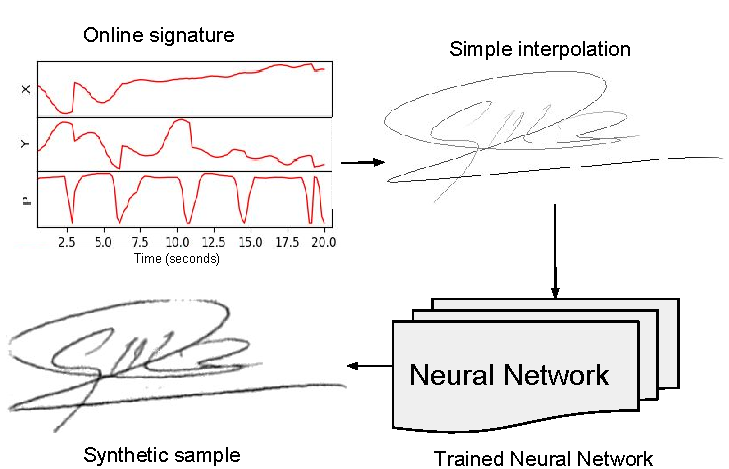
\includegraphics[width=3.6in]{method}
	% where an .eps filename suffix will be assumed under latex,
	% and a .pdf suffix will be assumed for pdflatex; or what has been declared
	% via \DeclareGraphicsExtensions.
	\caption{The proposed approach diagram and an example of the synthetic signature generation.}
	\label{fig_method}
\end{figure}



\section{Online to Offline Training Data}
In order to train our Neural Network to perform the approximation task of ``online to offline conversion,'' we need both the online version of a manuscript containing the trajectory and pressure information mapped to the respective resulting offline representation, as in Figure \ref{fig:offon}. Of course the mapping is a major problem since the two acquisition systems (digitizing tablet and optical scanner) process the writing signal separately, each having its particular parameters (Cartesian axis, scale, etc.). 

Moreover, the acquisition phase of such dual dataset requires some extra steps. A paper form must be placed over a digital tablet to be filled with an electronic ink-pen. Then, the dynamic data is captured through the tablet, and the paper form might be scanned to provide the offline image, Figure \ref{fig:dualonoff} illustrates this setup. Thereby, two complementary files are available. One contains the dynamic information, and the other one is the digital image of this piece of handwritten signature produced by the scanner. 
\begin{figure}[!htb]
\centering
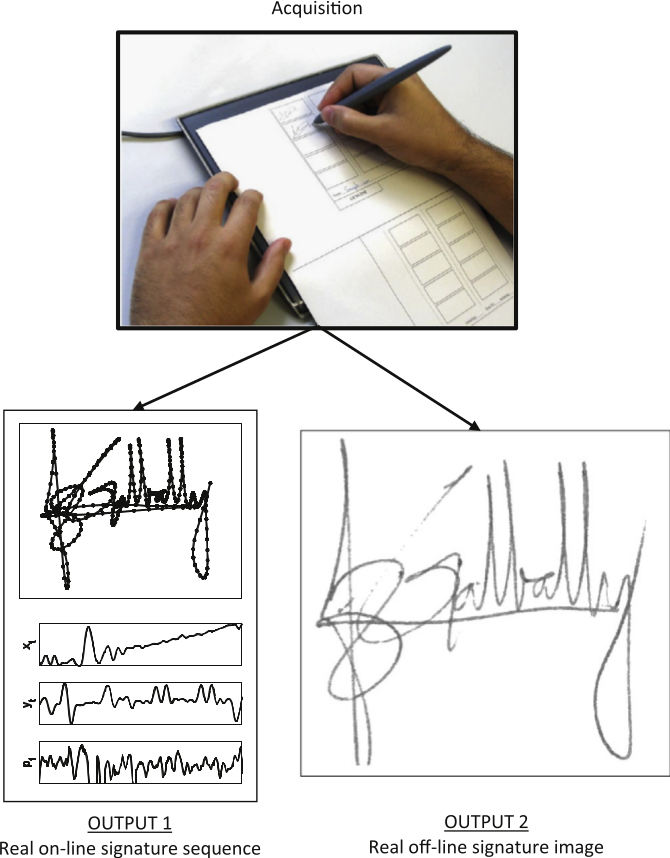
\includegraphics[width=0.7\textwidth]{dualonoff}

\caption{An user signing on a paper placed over a digitizing tablet. This way, the dynamic and static versions of the same signature are acquired simultaneously. Figure extracted from \cite{galbally2015line}}
\label{fig:dualonoff}
\end{figure}

In order to project the online signature in the respective offline version, these two types of information should be available within the same coordinate system, with the same origin, the same resolution, and orientation. However, as the two acquisition systems (tablet and scanner) are processing the writing separately and with their particular parameters, this assumption is not satisfied directly. Geometrical transformations have to be applied to compensate for these differences. To the best of our knowledge, however, the creators of the publicly available dual modal signature datasets \cite{biosecurid, biomet, myidea, sigcomp2009, sigma, sigwicomp2013, sigwicomp2015} had not this characteristic satisfied. As it can be seen in Figure \ref{fig:onoff}, both of the representations of the signatures do not match if we plot it in a single image.

\begin{figure}[!htb]
\centering
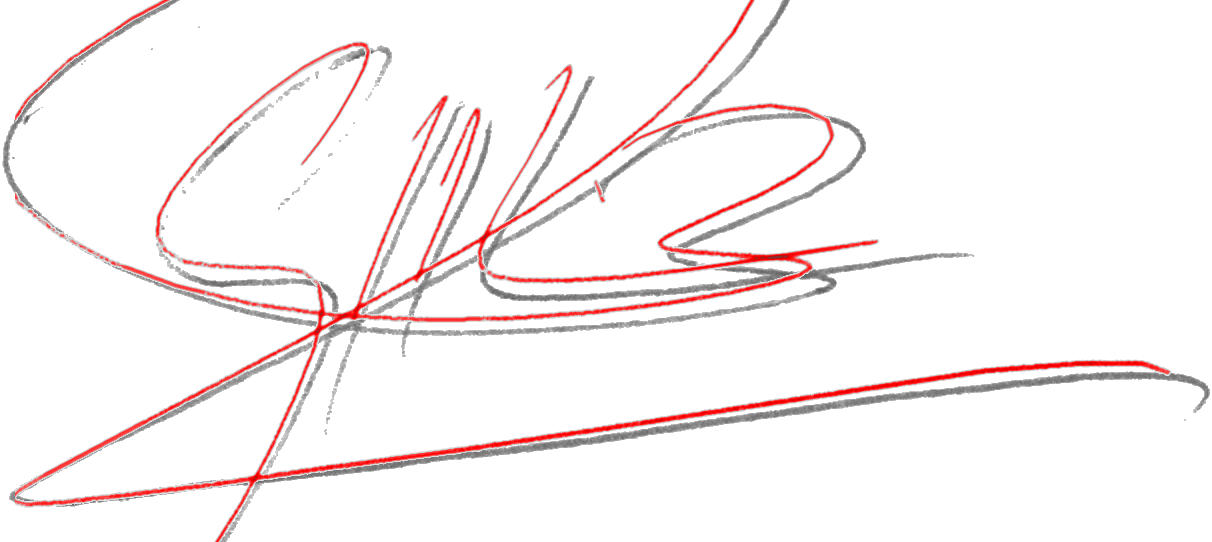
\includegraphics[width=0.5\textwidth]{onoff}
% where an .eps filename suffix will be assumed under latex, 
% and a .pdf suffix will be assumed for pdflatex; or what has been declared
% via \DeclareGraphicsExtensions.
\caption{A sample from the BiosecurID dataset. Here we can see that the online signature (interpolated in red) can not be projected in the respective offline version.}
\label{fig:onoff}
\end{figure}

The dual domain IRONOFF \cite{viard1999ireste} handwriting dataset was thus used to train our model. Besides acquiring both domains of the handwriting manuscript, the online data is mapped to the same coordinate system of the offline data, as shown in Figure \ref{fig:ironoff-mapped}, the interpolated online data is shown in white. Using this dataset, we make the fair assumption that a handwritten signature is a manuscript. With that in mind, we expect that even if the network was trained on handwriting manuscripts, it would work for online signatures to generate its static version.

The IRONOFF dataset contains a total of 23000 mapped online and offline samples of the manuscripts. The offline handwriting signals have been sampled with a spatial resolution of 300 dots per inch (DPI), with 8 bits per pixel (256 gray level).

\begin{figure}[!htb]
\centering

\includegraphics{ironoff-mapped}
% where an .eps filename suffix will be assumed under latex, 
% and a .pdf suffix will be assumed for pdflatex; or what has been declared
% via \DeclareGraphicsExtensions.
\caption{An offline manuscript mapped with the respective online trajectory. Image extracted from \cite{viard1999ireste}.}
\label{fig:ironoff-mapped}
\end{figure}


\section{Preprocessing}
%Copy and paste
During the training of our FCN model, two 2D matrices are needed, the input and output. The input is the online information of the manuscript, and the output is the expected offline representation.

In order to create a 2D representation of the dynamic information of the manuscript, we create a simple linear interpolated version of the time-series ($x_{t}, y_{t}, p_{t}$) using the Bresenham line algorithm \cite{bresenham} to obtain the 8-connected sequences. As a result, we get an image in which the trajectory of the signature is represented by one pixel, where the pixel intensity is the pressure information.

Since the neural network expect inputs and outputs of a fixed size and the manuscripts shape vary significantly in the IRONOFF (they range from samples of width x height size of 167x214 to larger samples of size 548x215 pixels), we convert it to a fixed size. We follow an approach similar to what was previously proposed in the literature, e.g., \cite{pourshahabi2009offline}. First, we normalize the images to the largest image size, by padding the images with white background. Then, we center the manuscript in a canvas of size 548x215 pixels (the largest sample size in the dataset), aligning the center of mass of the sample to the center of the image. Finally, we rescale the images, using a bilinear interpolation, to 383x150 pixels, i.e., 70\% of the canvas size, maintaining the aspect ratio of the original sample. This size was chosen to be large enough to keep details from the pen strokes in the manuscript.

Besides resizing the images to a standard size, we also performed the following pre-processing steps:
\begin{itemize}
\item Inverted the images: we inverted the images so that the white background corresponded to pixel intensity 0. 
\item Normalized the input: we normalized the input to the
neural network by dividing each pixel by the standard
deviation of all pixel intensities. We do not normalize the data to have mean 0 (another common pre-processing step) since we want the
background pixels to be zero-valued.
 
\end{itemize}

Figure \ref{fig_ironoff} shows what is the result of the preprocessed input and the groundtruth being fed to the neural network during the training phase.



\begin{figure}[!htpb]
\centering
 \subfloat[input]{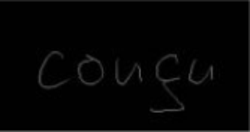
\includegraphics[width=2.0in]{input-ironoff}} 
\hspace*{0.5in} % separation between the subfigures
\subfloat[ground truth] {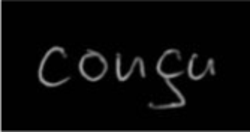
\includegraphics[width=2.0in]{gt-ironoff}}
\caption{Preprocessed data used during the training phase. (a) is the interpolated online sample, used as input and (b) is the expected prediction from the neural network, the ground truth. } \label{fig_ironoff}
\end{figure}



\section{Neural Network Model}

Our model is based on the fully convolutional neural network architecture, adopted to learn an end-to-end nonlinear mapping from online representation to the static image. Our Neural Network model is fed with the interpolated online sample pressure information and we expect the respective offline sample on the output, i.e., the input is the pressure information and the desired output is the static manuscript.

We use a simplified architecture based on the one proposed in \cite{long2015fully}. The expectation is that by learning to transform between online information to offline manuscripts, the network will learn convolution filters that are relevant to synthesize offline signatures based on the online sample.

Our convolutions architecture is a simplified version of the FCN-VGG \cite{long2015fully, simonyan2014very} and the transposed convolutions were symmetric to the convolution operations. We used a simplified version because during some initial tests we observed that the capacity of the original network architecture seemed to be too large for the problem at hand, particularly considering the amount of convolutional operations. We observed that the model was not learning useful transformations on the first few epochs. We obtained better results with the simplified architecture presented in Table \ref{table:cnn-arch}. 

For the purpose of replicating our experiment, we provide the list of the parameters used in our tests. Table \ref{table:cnn-arch} lists the definition of the FCN layers. For convolution and transpose convolution layers, we list the size as NxHxW where N is the number of filters, H is the height and W are the width of the layer window.

\begin{table}[!htb]
\renewcommand{\arraystretch}{1.3}
\caption{Summary of the CNN Layers}
\centering
\begin{tabular}{|l|l|}
\hline
\textbf{Layer}        & \textbf{Size} \\ \hline
Convolution           & 16x3x3        \\ \hline
Convolution           & 32x3x3        \\ \hline
Convolution           & 32x3x3        \\ \hline
Convolution           & 64x3x3        \\ \hline
Transpose Convolution & 64x3x3        \\ \hline
Transpose Convolution & 32x3x3        \\ \hline
Transpose Convolution & 32x3x3        \\ \hline
Transpose Convolution & 16x3x3        \\ \hline
\end{tabular}
\label{table:cnn-arch}
\end{table}

We used Leaky Rectified Linear Units (LReLUs) as the activation function for all convolutional layers. We also tried the Rectified Linear Units (ReLUs) but, although not performing extensive tests, we observed that on the first ten epochs the Neural Network seemed to be converging faster with the LReLUs. 

For every convolutional layer we use a stride (the distance between applications of the convolution operation) of 2x2, following what was observed by \cite{springenberg2014striving} that we can remove each pooling layer and increase the stride of the convolutional layer that preceded it accordingly. We pad the input for every layer with 0 evenly left and right and we initialize the weights of the model using the technique proposed by Glorot \textit{et al}\cite{glorot2010understanding}, and the biases to 0. 

We trained the model using the Adam optimizer to minimize the minimum squared error (MSE) loss for 100 epochs, using a learning rate of 0.001, and mini-batches of size 16. We used 22000 samples from the IRONOFF to train the model and another 1000 samples as validation data. The network was trained using the library Tensorflow and took around five days to train on a GTX 670 GPU.

\section{Training Results}
The MSE loss on the validation set over the 100 training epochs can be seen in Figure \ref{fig:trainingMSE}. We can see that the loss was varying from around 0.002 to 0.001 from epoch 20 until the last epoch. Figure \ref{fig:resultingsamples} shows a visual representation of the predictions, alongside the expected output. 
\begin{figure}[!htb]
\centering
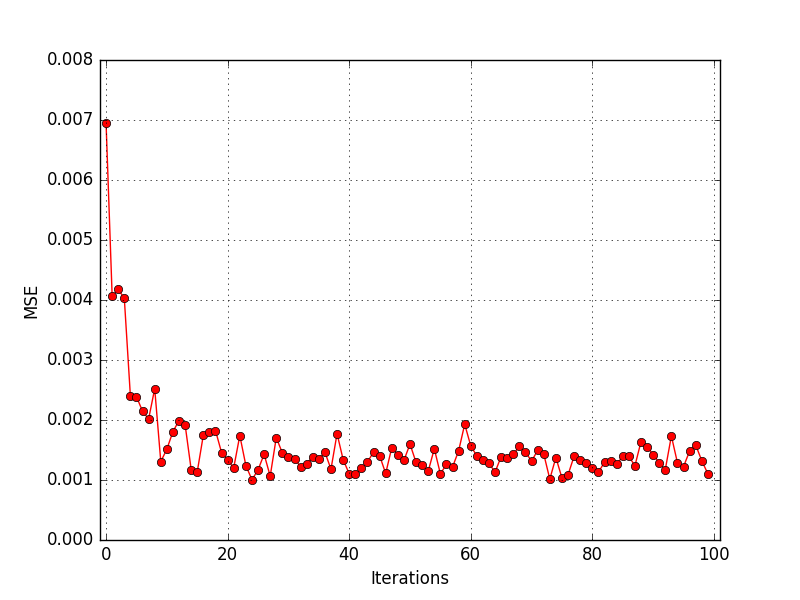
\includegraphics[width=0.8\textwidth]{iterations}
% where an .eps filename suffix will be assumed under latex, 
% and a .pdf suffix will be assumed for pdflatex; or what has been declared
% via \DeclareGraphicsExtensions.

\caption{Iterations versus validation loss.}
\label{fig:trainingMSE}

\end{figure}

\begin{figure}[!htpb]
\centering
\subfloat{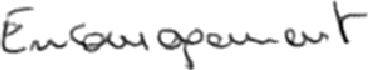
\includegraphics[scale=0.5]{samples/0}} 
\hspace*{0.4in} % separation between the subfigures
\subfloat{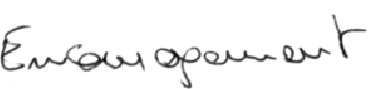
\includegraphics[scale=0.5]{samples/00}}
\\
\subfloat{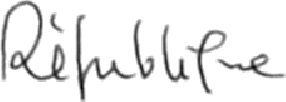
\includegraphics[scale=0.5]{samples/4}} 
\hspace*{0.4in} % separation between the subfigures
\subfloat{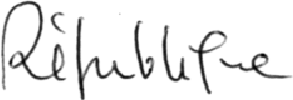
\includegraphics[scale=0.5]{samples/04}}
\\
\subfloat{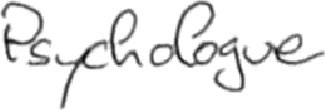
\includegraphics[scale=0.5]{samples/10}} 
\hspace*{0.4in} % separation between the subfigures
\subfloat{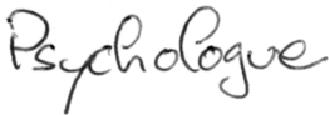
\includegraphics[scale=0.5]{samples/010}}
\\
\subfloat{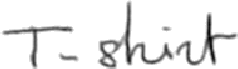
\includegraphics[scale=0.5]{samples/23}} 
\hspace*{0.4in} % separation between the subfigures
\subfloat{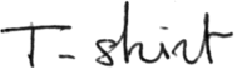
\includegraphics[scale=0.5]{samples/023}}
\\
\addtocounter{subfigure}{-8}
\subfloat[Synthetic Handwritten Manuscript]{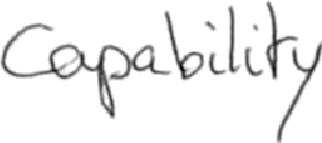
\includegraphics[scale=0.5]{samples/30}}
\hspace*{0.4in} % separation between the subfigures
\subfloat[Expected Real Manuscript - Groundtruth]{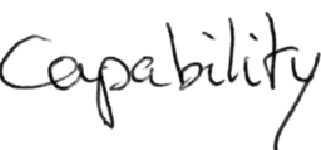
\includegraphics[scale=0.5]{samples/030}} 


\caption{A not cherry-picked selection of synthetic manuscripts produced using our proposed method alongside the expected output, i.e. the groundtruth.} \label{fig:resultingsamples}
\end{figure}

We can observe that the synthetic samples are similar to the expected output, however, in order to make an objective evaluation of the quality of the synthetic generation, in the context of handwritten signatures, we performed a machine-oriented evaluation. In the next chapter, we describe the protocol we followed and then we report an objective measure of the quality of our proposed method based on this experimental setup.
